\documentclass{standalone}
\usepackage{tikz}
\usepackage{textcomp}

\begin{document}

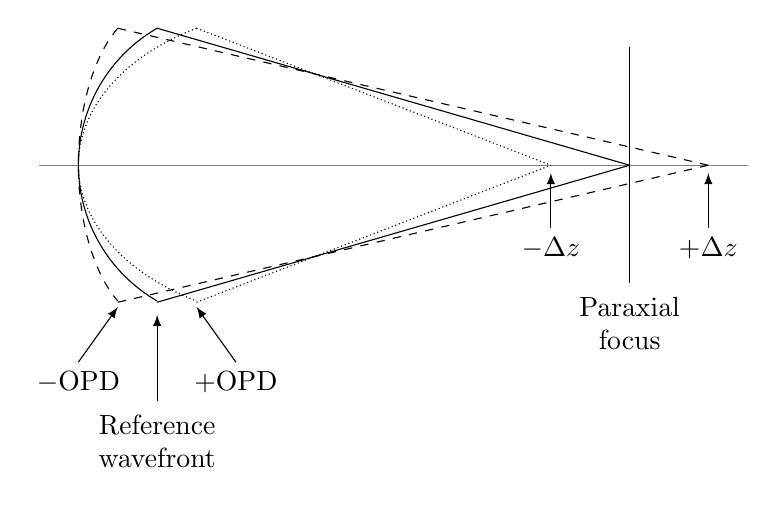
\begin{tikzpicture}

    \draw [gray] (-1.5,0) -- (7.5,0);
   
    \draw (0,1.74) arc [
        start angle=120,
        end angle=240,
        x radius=2,
        y radius=2];

    \draw (0,1.74) -- (6,0);
    \draw (0,-1.74) -- (6,0);

    \draw [latex-] (0, -1.9) -- (0,-3);
    \node [below] at (0, -3) {\begin{tabular}{c}Reference\\wavefront\end{tabular}};
    
        \draw (6, 1.5) -- (6,-1.5);
    \node [below] at (6, -1.5) {\begin{tabular}{c}Paraxial\\focus\end{tabular}};

    \draw [densely dotted] (0.5,1.74) arc [
        start angle=120,
        end angle=240,
        x radius=3,
        y radius=2];
    
    \draw [densely dotted] (0.5,1.74) -- (5,0);
    \draw [densely dotted] (0.5,-1.74) -- (5,0);
    
    \draw [latex-] (0.5,-1.8) -- (1,-2.5);
    \node [below] at (1,-2.5) {$+\mbox{OPD}$};
    
    \draw [latex-] (5,-0.1) -- (5,-0.8);
    \node [below] at (5,-0.8) {$-\Delta z$};

    \draw [dashed] (-0.5,1.74) arc [
        start angle=120,
        end angle=240,
        x radius=1,
        y radius=2];
    
    \draw [dashed] (-0.5,1.74) -- (7,0);
    \draw [dashed] (-0.5,-1.74) -- (7,0);

    \draw [latex-] (-0.5,-1.8) -- (-1,-2.5);
    \node [below] at (-1,-2.5) {$-\mbox{OPD}$};
    
    \draw [latex-] (7,-0.1) -- (7,-0.8);
    \node [below] at (7,-0.8) {$+\Delta z$};
    
\end{tikzpicture}
\end{document}
